\documentclass[tikz,border=1mm]{standalone}

\usepackage[latin1]{inputenc}
\usepackage[T1]{fontenc}
\usepackage{lmodern}

\usetikzlibrary{positioning,circuits.logic.US,arrows.meta}

\begin{document}

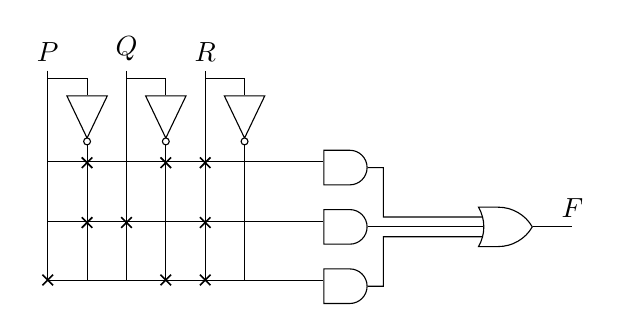
\begin{tikzpicture}[%
    circuit logic US,
    tiny circuit symbols,
    every circuit symbol/.style={fill=white, draw},
    node distance=3mm and 0mm,
    branch/.style={fill,shape=circle,minimum size=3pt,inner sep=0pt}]

    \coordinate[label=above:$P$] (a) at (0,0);
    \coordinate[label=above:$Q$] (b) at (1,0);
   
    \coordinate[label=above:$R$] (d) at (2,0);

    \node[not gate, rotate=-90] at ($(a)+(0.5,-.5)$) (Nota) {};
    \node[not gate, rotate=-90] at ($(d)+(0.5,-.5)$) (Notd) {};
     \node[not gate, rotate=-90] at ($(b)+(0.5,-.5)$) (Notb) {};

    \node[and gate, logic gate inputs=nn, anchor=north west] at ($(d)+(1.5,-1)$) (and1) {};
    \node[and gate, logic gate inputs=nn, below=of and1]  (and2) {};
    \node[and gate, below=of and2] (And3) {};
 \node[or gate US, draw, logic gate inputs=nnn ] at ($(and2)+(2,0)$) (or) {};
   
   \draw (or.output) -- ([xshift=0.5cm]or.output) node[above] {$F$};
    
    

    \draw ($(a)+(0,-1mm)$)-|(Nota);
    \draw ($(d)+(0,-1mm)$)-|(Notd);
     \draw ($(b)+(0,-1mm)$)-|(Notb);
   
     

 \draw (Nota)|-(and1.input 1);
   
    \draw (Nota)|-(and2.input 1);
  
     \draw (Nota)|-(And3.input 1);
       
     \draw (a)|-(and2.input 1); 
      \draw (a)|-(and1.input 1);
       \draw (a)|-(And3.input 1); 
   
   
   
    
      \draw (Notb)|-(and1.input 1);
      \draw (Notb)|-(And3.input 1);
      \draw (Notb)|-(and2.input 1); 
     \draw (b)|-(And3.input 1);
     
     
   
       \draw (d)|-(And3.input 1);
       \draw (Notd)|-(And3.input 1);
   
    \draw (Notd)|-(and1.input 1);
  

\draw (and1)--++(0:5mm)|-(or.input 1);
\draw (and2.output)|-(or.input 2);
  \draw (And3)--++(0:5mm)|-(or.input 3);

  
  
\draw[-{ Rays[n=4][black,length=1mm,width=1mm]},semithick] (1,-1.85);    
\draw[-{ Rays[n=4][black,length=1mm,width=1mm]},semithick] (2,-1.85);  
\draw[-{ Rays[n=4][black,length=1mm,width=1mm]},semithick] (0.5,-1.85);  


\draw[-{ Rays[n=4][black,length=1mm,width=1mm]},semithick] (0,-2.58);
\draw[-{ Rays[n=4][black,length=1mm,width=1mm]},semithick] (1.5,-2.58);
\draw[-{ Rays[n=4][black,length=1mm,width=1mm]},semithick] (2,-2.58);

\draw[-{ Rays[n=4][black,length=1mm,width=1mm]},semithick] (0.5,-1.09);
\draw[-{  Rays[n=4][black,length=1mm,width=1mm]},semithick] (1.5,-1.09);
  \draw[-{ Rays[n=4][black,length=1mm,width=1mm]},semithick] (2,-1.09);
 
\end{tikzpicture}
\end{document} 